%% Compiler: XeLaTeX

\documentclass[tikz,border=0pt,11pt]{standalone}%
\usepackage{tikz-cd}
\usepackage{ifthen}
\usepackage{amsmath}

\usetikzlibrary{arrows,calc,intersections,shapes}


\begin{document}

%---------------------------------------------------------------
        %% MLP_Bias-Neuron
        %-----------------------------------------
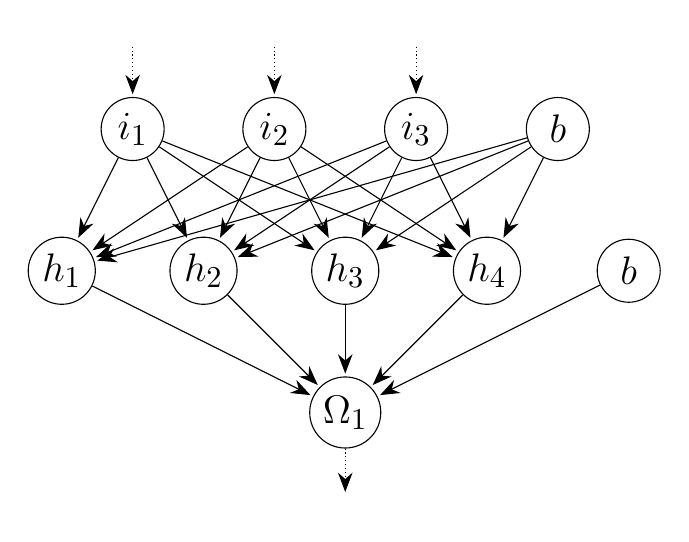
\begin{tikzpicture}[>=stealth', node distance=\layersep cm, shorten >=1pt]
        \def\layersep{1.8}            % vertikal distance between the layers
        \def\neuronsep{1.8}         % Horizontal distance between neurons
        \def\dlsize{2}            % distance between node and layer lable
        \def\inout{\layersep*.65}   % Size of in- and output-arrow
        \def\siz{.8}                % neuronsize
        \def\y{5}                   % Start of the most upper layer
        \def\ni{3}                  % Amount of input neurons
        \def\nh{4}                  % Amount of hidden neurons
        \def\no{1}                  % Amount of output neurons
        \tikzstyle{neuron}=[circle,draw=black,minimum size=\siz cm,inner sep=2pt]
        \tikzstyle{annot} = [text width=6em, text centered]
        \tikzset{fontscale/.style = {font={\fontsize{#1pt}{#1pt}\selectfont}}}

        \newcommand{\neurono}[2][]{
            \node[neuron,circle split,inner sep=2pt] (#1) at (#2)
                    {\includegraphics[width=0.225cm]{Bilder/Sigma.png} \nodepart{lower} \includegraphics[width=0.225cm]{Bilder/sigma.png}};
        }
        % Draw the left input layer nodes
            \foreach \name / \xn in {1,...,\ni}{
            % This is the same as writing \foreach \name / \y in {1/1,2/2,3/3,4/4}
                \node[neuron,fontscale=15] (Il-\name) at (\xn*\neuronsep-\neuronsep,\y) {$i_{\xn}$};
                \node[above of=Il-\name, node distance=\inout cm] (Inl-\name) {};
                \draw [->,arrows={-Stealth[length=7pt]},densely dotted] (Inl-\name) edge (Il-\name);
            }
            \node[neuron,fontscale=15] (Il-b) at ({(\ni+1)*\neuronsep-\neuronsep},\y) {$b$};
        % Draw the hidden layer node
            \foreach \name / \xn in {1,...,\nh}{
                \node[neuron,fontscale=15] (Hl-\xn) at ({(\ni-1)*\neuronsep/2-\neuronsep/2*(\nh-1)+(\xn-1)*\neuronsep},\y-\layersep) {$h_{\xn}$};
                \node[node distance=\inout cm, below of=Hl-\xn] (Hnl) {};
                
                \ifthenelse{\xn=\nh}{ 
                    \node[neuron,fontscale=15, right of=Hl-\nh] (Hl-b)  {$b$};
                }{}
        % Connect every node in the inner layer with the hidden layer
            \draw [->,arrows={-Stealth[length=7pt]}] (Il-b) edge (Hl-\xn);
            \foreach \source in {1,...,\ni}
                \draw [->,arrows={-Stealth[length=7pt]}] (Il-\source) edge (Hl-\xn);
                }
            \node[neuron,fontscale=15,below of=Hl-3 ] (Ol-1) {$\Omega_{1}$};
            \node[node distance=\inout cm, below of=Ol-1] (Onl) {};
            \draw [->,arrows={-Stealth[length=7pt]},densely dotted] (Ol-1) edge (Onl);
        % Connect every node in the hidden layer with the output layer
            \draw [->,arrows={-Stealth[length=7pt]}] (Hl-b) edge (Ol-1);
            \foreach \source in {1,...,\nh}
                \draw [->,arrows={-Stealth[length=7pt]}] (Hl-\source) edge (Ol-1);

\end{tikzpicture}


\end{document}